\section{Results}\label{sec:results}
\begin{table*}[!t]
\caption{Discrimination under P1: mean AUROC over 25 test folds. Bold: highest mean (ties within 0.0005). Upper block: literature-standard methods; lower block: state-of-the-art learners, HARBOR and PredictX.}
\label{tab:auroc}
\centering\small
\begin{tabular}{lccccc}
\toprule
Model & Coronary & Diabetes & Breast & Liver & Kidney\\
\midrule
\tablebody{generated/tab_auroc.tex}
\bottomrule
\end{tabular}
\end{table*}

\begin{table*}[!t]
\caption{Mean paired AUROC difference between PredictX and each comparator over 25 folds (coronary: PredictX with cross-site training). $^{\uparrow}$: 95\% Nadeau--Bengio interval entirely above zero; $^{\downarrow}$: entirely below zero. Last column: wins/ties/losses.}
\label{tab:paired}
\centering\small
\begin{tabular}{lcccccc}
\toprule
Comparator & Coronary & Diabetes & Breast & Liver & Kidney & W/T/L\\
\midrule
\tablebody{generated/tab_paired.tex}
\bottomrule
\end{tabular}
\end{table*}

\subsection{Benchmark}
Table~\ref{tab:auroc} reports mean AUROC under P1. PredictX attains the highest AUROC on coronary disease (0.915 with cross-site training) and ties at 1.000 on chronic kidney disease. On diabetes (0.846), breast malignancy (0.994) and liver disease (0.750) it is within 0.002 of the best learner, TabPFN v2. The strongest literature-standard method varies by cohort: logistic regression for coronary and liver disease, tuned XGBoost for diabetes, the SVM for breast malignancy and random forest for kidney disease.

Table~\ref{tab:paired} tests every pairwise difference with corrected intervals. Across the 50 cohort--comparator pairs, PredictX is significantly better in 12 and significantly worse in none. It significantly outperforms naive Bayes on three cohorts; $k$-NN, random forest and the MLP on two; and logistic regression, tuned XGBoost and CatBoost on one each. Against the best literature-standard method of each cohort the mean differences are $+0.006$ for coronary disease (95\% CI $-0.010$ to $+0.021$), $+0.007$ for diabetes ($-0.003$ to $+0.017$), $+0.002$ for liver disease ($-0.019$ to $+0.023$) and $-0.001$ for breast malignancy ($-0.002$ to $+0.001$) (Fig.~\ref{fig:delta}).

\begin{figure}[!t]
\centering
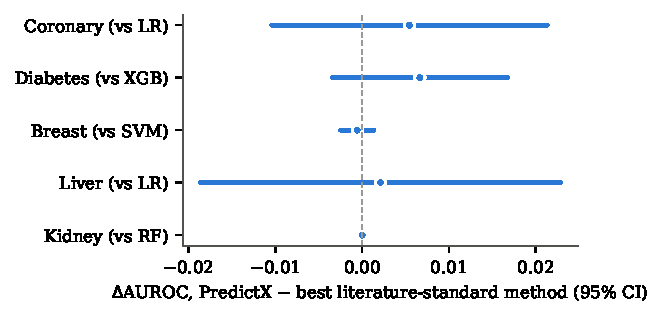
\includegraphics[width=\columnwidth]{generated/fig_delta.pdf}
\caption{PredictX minus the best literature-standard method of each cohort: mean paired AUROC difference with 95\% Nadeau--Bengio interval over 25 folds.}
\label{fig:delta}
\end{figure}

Table~\ref{tab:accuracy} compares accuracy at the 0.5 threshold and the Brier score with the best literature-standard method of each cohort. PredictX has the lower Brier score on all five cohorts (coronary 0.117 versus 0.119, diabetes 0.153 versus 0.156, breast 0.025 versus 0.026, liver 0.171 versus 0.173, kidney 0.001 versus 0.009), consistent with Proposition~\ref{prop:ens}, and its accuracy ranges from 71.9\% (liver) to 100\% (kidney). Among all eleven models, PredictX has the lowest Brier score on liver disease and the second lowest, after TabPFN v2, on the other four cohorts.

\begin{table}[!t]
\caption{Accuracy (\%, threshold 0.5) and Brier score: best literature-standard method versus PredictX (P1, 25 folds)}
\label{tab:accuracy}
\centering\footnotesize
\setlength{\tabcolsep}{3pt}
\begin{tabular}{llcccc}
\toprule
& & \multicolumn{2}{c}{Best standard} & \multicolumn{2}{c}{PredictX}\\
Cohort & Method & Acc. & Brier & Acc. & Brier\\
\midrule
\tablebody{generated/tab_accuracy.tex}
\bottomrule
\end{tabular}
\end{table}

\subsection{Comparison with published results}
Table~\ref{tab:published} places our results beside the TabPFN benchmark \cite{tabpfn}, in which every baseline received 60 minutes of hyperparameter optimization per split, under its 50/50 protocol (P2). PredictX exceeds the best published value on breast malignancy (0.9953 versus 0.9940) and liver disease (0.7438 versus 0.7412), and its TabPFN v2 member exceeds the best published diabetes value (0.8463 versus 0.8427). The PredictX ensemble scores 0.8402 on diabetes under this protocol.

\begin{table*}[!t]
\caption{ROC AUC under the published 50/50 protocol (five splits). Left: values published by Hollmann et al.\ \cite{tabpfn} (n.e.: without ensembling). Right: this work. Bold: row maximum.}
\label{tab:published}
\centering\small
\begin{tabular}{l|cccccc|ccc}
\toprule
& \multicolumn{6}{c|}{Published \cite{tabpfn}} & \multicolumn{3}{c}{This work}\\
Cohort & CatBoost & XGBoost & AutoGluon & TabPFN n.e. & TabPFN & TabPFN+AutoGluon & TabPFN v2 & CatBoost & PredictX\\
\midrule
\tablebody{generated/tab_published.tex}
\bottomrule
\end{tabular}
\end{table*}

\subsection{Ablations}
\begin{table}[!t]
\caption{Leave-one-member-out: AUROC of PredictX minus PredictX without the listed member (mean over 25 folds).}
\label{tab:members}
\centering\footnotesize
\begin{tabular}{lcccc}
\toprule
Cohort & TabPFN v2 & CatBoost & LR & HARBOR\\
\midrule
\tablebody{generated/tab_members.tex}
\bottomrule
\end{tabular}
\end{table}

\para{Ensemble members.}Removing a single member changes mean AUROC by at most 0.0023 (Table~\ref{tab:members}). The largest contributions are TabPFN v2 on diabetes ($+0.0023$), logistic regression on coronary disease ($+0.0018$) and TabPFN v2 on coronary disease ($+0.0014$); HARBOR contributes $+0.0009$ on diabetes.

\para{Cross-site training.}Adding the Hungarian, Swiss and VA Long Beach cohorts to every training fold raised the mean coronary AUROC of logistic regression ($+0.002$), CatBoost ($+0.001$), HARBOR ($+0.005$) and PredictX ($+0.001$), and left TabPFN v2 at 0.913 (Table~\ref{tab:crosssite}). HARBOR, whose typed tokens represent the auxiliary cohorts' missing tests explicitly, gains most.

\begin{table}[!t]
\caption{Cross-site training on coronary disease: mean AUROC on Cleveland test folds when training on Cleveland only and on Cleveland plus the three auxiliary cohorts.}
\label{tab:crosssite}
\centering\footnotesize
\begin{tabular}{lccc}
\toprule
Learner & Cleveland & + auxiliary & $\Delta$\\
\midrule
\tablebody{generated/tab_crosssite.tex}
\bottomrule
\end{tabular}
\end{table}

\para{Availability channel.}Table~\ref{tab:missingness} reports protocol P4. Under MCAR the pattern is independent of the label by construction (mask-only AUROC 0.573 on WDBC and 0.433 on ILPD for the injected realization), and the three HARBOR variants lie within 0.005 of each other. Under self-masking MNAR on WDBC, where the mask alone predicts malignancy with AUROC 0.969, the variants that represent availability reach 0.979 (two-channel) and 0.981 (mask-concat), against 0.966 for the value-only encoder; the two-channel minus value-only difference is $+0.013$ (95\% CI $-0.001$ to $+0.027$). On ILPD, where the injected pattern is weakly informative (mask-only AUROC 0.626), the variants lie within 0.002 of each other.

\begin{table*}[!t]
\caption{Controlled missingness (P4; 40\% of every numeric feature removed). Mask only: logistic regression on the missingness pattern. HARBOR variants are single-member models. Last two columns: paired AUROC differences with corrected 95\% intervals over 25 folds.}
\label{tab:missingness}
\centering\small
\resizebox{\textwidth}{!}{%
\begin{tabular}{llccccccc}
\toprule
Data & Mech. & Mask only & LR & Value-only & Mask-concat & Two-channel & Two-ch.\ $-$ Value-only & Two-ch.\ $-$ Mask-concat\\
\midrule
\tablebody{generated/tab_missingness.tex}
\bottomrule
\end{tabular}}
\end{table*}

\subsection{Value-of-information test acquisition}
\begin{figure}[!t]
\centering
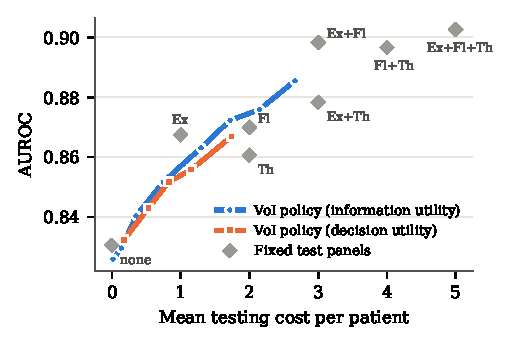
\includegraphics[width=\columnwidth]{generated/fig_acquisition.pdf}
\caption{Testing cost versus AUROC for coronary disease (P3, 25 folds). Grey diamonds: fixed test panels (Ex exercise ECG, Fl fluoroscopy, Th thallium scintigraphy). Lines: value-of-information policies over a sweep of $\lambda$.}
\label{fig:acquisition}
\end{figure}

Fig.~\ref{fig:acquisition} and Table~\ref{tab:acquisition} report protocol P3. With $\lambda=0$, the information-utility policy orders 1.53 of the three tests per patient at a mean cost of 2.66, against 5.0 for the full panel, and reaches AUROC 0.886 and accuracy 82.2\%, against 0.903 and 83.2\% with every test: 98\% of the full-panel AUROC at 53\% of the testing cost. Increasing $\lambda$ traces a monotone frontier down to the baseline work-up (AUROC 0.830 at zero cost). Above a mean cost of 0.2 the information utility attains a higher AUROC than the decision utility at matched cost, because the decision utility values a test exactly when its result can change the current decision. Among fixed panels, exercise ECG with fluoroscopy reaches 0.898 at cost 3.0.

\begin{table}[!t]
\caption{Test-acquisition policies for coronary disease (P3): mean cost, tests per patient, AUROC and accuracy (\%).}
\label{tab:acquisition}
\centering\footnotesize
\setlength{\tabcolsep}{3pt}
\begin{tabular}{lcccc}
\toprule
Policy & Cost & Tests & AUROC & Acc.\\
\midrule
\tablebody{generated/tab_acquisition.tex}
\bottomrule
\end{tabular}
\end{table}

\subsection{Deployed models on the clinical input forms}\label{sec:deployed}
Table~\ref{tab:web} reports the deployed configuration: PredictX trained on exactly the form fields of Table~\ref{tab:forms}, evaluated under P1. The deployed models reach AUROC 0.915 for coronary disease, 0.846 for diabetes, 0.994 for breast malignancy, 0.741 for liver disease and 0.996 for chronic kidney disease, with accuracies between 70.2\% and 97.8\%. With seven routine urine and blood-pressure fields, the kidney model retains an AUROC of 0.996 relative to 1.000 with all 24 predictors.

\begin{table}[!t]
\caption{Deployed configuration: PredictX on the form fields (P1, 25 folds), with the best literature-standard method on the same fields.}
\label{tab:web}
\centering\footnotesize
\setlength{\tabcolsep}{3pt}
\begin{tabular}{lcccll}
\toprule
& & \multicolumn{2}{c}{PredictX} & \multicolumn{2}{c}{Best standard}\\
Endpoint & Fields & AUROC & Acc. & Method & AUROC\\
\midrule
\tablebody{generated/tab_web.tex}
\bottomrule
\end{tabular}
\end{table}
